\documentclass[runningheads]{llncs}
\usepackage[T1]{fontenc}
\usepackage{graphicx}
\usepackage{amsmath,amssymb}
\usepackage{booktabs}
\usepackage{array}
\usepackage{tikz}
\usetikzlibrary{arrows.meta,positioning,fit,calc}
\usepackage{hyperref}
\usepackage{url}

% Space-efficient Springer LNCS float and spacing parameters
\setlength{\textfloatsep}{4pt plus 1pt minus 1pt}
\setlength{\floatsep}{4pt plus 1pt minus 1pt}
\setlength{\intextsep}{4pt plus 1pt minus 1pt}
\setlength{\abovecaptionskip}{2pt}
\setlength{\belowcaptionskip}{1pt}
\setlength{\tabcolsep}{2.5pt}
\raggedbottom

\begin{document}

\title{Autonomous Credit Intelligence: An Event-Driven, Self-Healing Multi-Agent Framework for Real-Time B2B Risk Assessment}

\titlerunning{ACIS-X: Multi-Agent Credit Intelligence Framework}

\author{Nikhil Nagendra\inst{1} \and
Pallavi K V\inst{1} \and
Johan K George\inst{1} \and
Nitin Bharadwaj MVS\inst{1} \and
Prasanna B Acharya\inst{1} \and
Bhoomi Joshi\inst{1}}

\authorrunning{N.~Nagendra et al.}

\institute{
Department of Computer Science and Engineering,\\
AMC Engineering College, 18th K.M. Bannerghatta Main Road,\\
Bengaluru 560083, Karnataka, India\\
\email{nikhilnag98@gmail.com}
}

\maketitle

\begin{abstract}
Intraday B2B credit monitoring requires continuous synthesis of payment behaviour, balance-sheet fundamentals, and litigation signals. Given the proprietary confidentiality of commercial enterprise trade ledgers, evaluating streaming credit architectures necessitates reproducible macroeconomic stress simulation. This paper presents ACIS-X, a reactive event-driven multi-agent framework on Apache Kafka that continuously maintains a live per-customer risk score. Specialized agents coordinate over partitioned Kafka topics across five core layers, an autonomous model governance plane, and a cross-cutting self-healing plane. ACIS-X combines native Kafka Exactly-Once Semantics (EOS) with idempotent database sinks, three-tier signal fusion, SHAP audit logging, streaming drift tracking via Population Stability Index (PSI), and heartbeat-driven recovery from committed offsets. Evaluated under an empirical jump-diffusion stress harness, ACIS-X demonstrates sub-50\,ms streaming latency (P95 16.2\,ms), near-linear consumer scaling, and autonomous fault recovery with storm prevention.
\end{abstract}

\keywords{Multi-agent systems \and Event-driven architecture \and Credit risk intelligence \and Apache Kafka \and Exactly-Once Semantics \and Self-healing systems}

\section{Introduction}
\label{sec:intro}
Enterprise credit risk monitoring demands continuous evaluation of payment dynamics, financial health, and litigation. While event streaming platforms like Apache Kafka~\cite{kreps2011kafka} enable real-time risk updates, recent LLM-based multi-agent systems~\cite{jajoo2025masca} introduce multi-second latencies ($>2$\,s) and non-deterministic outputs unsuitable for sub-50\,ms financial streaming subject to deterministic compliance controls. Conversely, conventional Kafka pipelines perform static transaction scoring without agentic autonomy or continuous drift governance.
A fundamental challenge in academic credit research is that real B2B invoice ledgers, trade terms, and defaults are confidential commercial secrets protected by strict enterprise NDAs. We therefore emphasize a clear separation between \textit{architectural validation} (the core contribution of this work) and \textit{empirical default forecasting}. We introduce ACIS-X (Autonomous Credit Intelligence System, Extended), an event-driven multi-agent framework grounded in the Actor model. The contributions are: (1) an event-driven multi-agent architecture on Kafka with autonomous self-healing and model governance; (2) Kafka stream-level Exactly-Once Semantics (EOS) combined with idempotent persistence and action deduplication for external sinks; (3) three-tier signal fusion integrating behavioural metrics, financial ratios, and litigation with deterministic risk policy guardrails; (4) streaming model governance inspired by SR~11-7 principles via PSI drift tracking and online challenger benchmarking; and (5) comprehensive systems benchmarks measuring throughput, partition scaling, consumer lag, P95/P99 latency, and fault recovery under a jump-diffusion stress harness. 

\section{Related Work}
\label{sec:related}
Corporate credit scoring, from classic Z-scores~\cite{altman1968financial} to explainable ML~\cite{chang2025explainable,nwafor2024hybrid}, relies primarily on offline batch feature stores incapable of capturing intraday delinquency transitions. While Kafka event sourcing is widely adopted for sub-second fraud scoring~\cite{kesarpu2025kafka,parnerkar2025eda}, existing streaming architectures evaluate isolated transactions rather than stateful, multi-source enterprise credit profiles combining balance-sheet ratios and court litigation. 
Recently, cognitive multi-agent frameworks like MASCA~\cite{jajoo2025masca} and Kubam's credit agent~\cite{kubam2026agentic} applied LLMs to qualitative risk assessment. However, their multi-second execution times and prompt non-determinism make them incompatible with high-throughput, low-latency ($<$50\,ms) streaming pipelines. In addition, existing microservice resilience mechanisms~\cite{beereddy2025selfhealing} recover at coarse container boundaries rather than providing granular per-agent heartbeat recovery with deterministic offset replay. As summarized in Table~\ref{tab:comparison}, ACIS-X bridges these paradigms: unlike cognitive MAS, it executes deterministically at sub-50\,ms latency; unlike standard streaming engines, it provides autonomous agent drift governance and offset-driven self-healing without requiring external compute clusters (e.g., Flink).

Table~\ref{tab:comparison} contrasts the operational and architectural characteristics of prior paradigms against ACIS-X. 

\begin{table}[htbp]
\caption{Architectural positioning across enterprise credit risk paradigms}
\label{tab:comparison}
\centering\scriptsize
\resizebox{\columnwidth}{!}{
\begin{tabular}{@{}lcccc@{}}
\toprule
\textbf{Dimension} & \textbf{Batch XAI~\cite{chang2025explainable}} & \textbf{Stream Risk~\cite{parnerkar2025eda}} & \textbf{Cognitive MAS~\cite{jajoo2025masca,kubam2026agentic}} & \textbf{ACIS-X (Ours)} \\
\midrule
Latency Profile & Hours -- Days & Sub-second ($<$1\,s) & Multi-second ($>$2\,s) & Sub-50\,ms (P95 16\,ms) \\
Signal Scope & Financial ratios & Single transaction stream & Text / financial reports & 3-tier (AR + Fin + Legal) \\
Execution Model & Periodic batch scripts & Stream processing & Deliberative LLM / MARL & Reactive event-driven MAS \\
Atomicity Guarantee & DB ACID transactions & At-least-once / EOS & None (stateless LLM) & Native Kafka EOS + PK \\
Fault Recovery & Cold process restart & Node failover & None / prompt retry & Heartbeat + offset resume \\
Drift Governance & Offline re-training & External metric dashboard & Manual prompt tuning & Streaming PSI + Challenger \\
\bottomrule
\end{tabular}
}
\end{table}

As shown in Table~\ref{tab:comparison}, ACIS-X uniquely occupies the intersection of streaming credit fusion, deterministic compliance, autonomous governance, and fine-grained agent recovery: specialized reactive agents exchange only Kafka events, fuse three signal families online, and resume autonomously from the last committed offset.

\section{System Architecture}
\label{sec:architecture}

ACIS-X maintains a live risk score for each customer $c_i$:
\begin{equation}
\mathcal{R}(c_i,t) = \mathcal{F}\bigl(\mathcal{B}(c_i,t),\;\mathcal{E}(c_i,t),\;\mathcal{L}(c_i,t)\bigr) \in [0,1],
\label{eq:risk}
\end{equation}
where $\mathcal{B}$ is behavioural history, $\mathcal{E}$ external financial indicators, and $\mathcal{L}$ litigation exposure. Design targets are sub-second processing, usable scores under partial signals, zero silent loss of committed work across restart, and idempotent duplicate handling.

The runtime architecture is illustrated in Figure~\ref{fig:arch}. The layers 1--4 sit on top of a common Apache Kafka event bus; layers 5 (persistence), 6 (model governance), and the system plane reside below. Agents only communicate via Kafka: Layer~1 deals with customers, invoices, payments, and behavioral indicators; Layer~2 uses financial APIs and litigation information to enrich data and aggregate signals; Layer~3 calculates payment risk and updates the compound score; Layer~4 performs credit policy and collections action; Layer~5 keeps track of system state; Layer~6 measures drift and assesses challenger models; the system plane manages time ticks, monitoring, self-healing, DLQ monitoring, and runtime placement.

\begin{figure}[htbp]
\centering
\resizebox{0.92\columnwidth}{!}{%
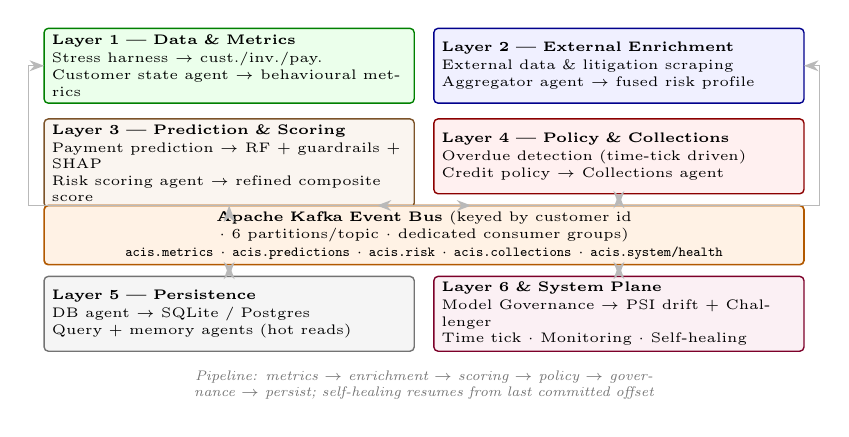
\begin{tikzpicture}[
  font=\tiny, >=Stealth,
  box/.style 2 args={
    draw=#1, fill=#2, line width=0.5pt, rounded corners=1.5pt,
    text width=4.5cm, minimum width=4.7cm, minimum height=0.95cm,
    align=left, inner sep=2pt, outer sep=0pt, anchor=north west
  },
  bus/.style={
    draw=orange!70!black, fill=orange!10, line width=0.6pt, rounded corners=1.5pt,
    minimum height=0.65cm, align=center,
    inner sep=2pt, outer sep=0pt, anchor=north west
  },
  arr/.style={<->, line width=0.5pt, draw=gray!55}
]
\def\gx{4.95} \def\gyA{0.00} \def\gyB{-1.15} \def\gyK{-2.25} \def\gyC{-3.15}

\node[box={green!50!black}{green!8}] (l1) at (0,\gyA) {%
  \textbf{Layer 1 --- Data \& Metrics}\\[0.5pt]
  Stress harness $\rightarrow$ cust./inv./pay.\\
  Customer state agent $\rightarrow$ behavioural metrics};

\node[box={blue!55!black}{blue!6}] (l2) at (\gx,\gyA) {%
  \textbf{Layer 2 --- External Enrichment}\\[0.5pt]
  External data \& litigation scraping\\
  Aggregator agent $\rightarrow$ fused risk profile};

\node[box={brown!65!black}{brown!8}] (l3) at (0,\gyB) {%
  \textbf{Layer 3 --- Prediction \& Scoring}\\[0.5pt]
  Payment prediction $\rightarrow$ RF + guardrails + SHAP\\
  Risk scoring agent $\rightarrow$ refined composite score};

\node[box={red!55!black}{red!6}] (l4) at (\gx,\gyB) {%
  \textbf{Layer 4 --- Policy \& Collections}\\[0.5pt]
  Overdue detection (time-tick driven)\\
  Credit policy $\rightarrow$ Collections agent};

\path let \p1=(l1.west), \p2=(l2.east) in
  node[bus, minimum width=\x2-\x1, text width=\x2-\x1-4pt] (k)
  at (\p1 |- 0,\gyK) {%
  \textbf{Apache Kafka Event Bus} (keyed by customer id $\cdot$ 6 partitions/topic $\cdot$ dedicated consumer groups)\\[0.5pt]
  \texttt{acis.metrics} $\cdot$ \texttt{acis.predictions} $\cdot$ \texttt{acis.risk} $\cdot$ \texttt{acis.collections} $\cdot$ \texttt{acis.system/health}};

\node[box={black!55}{black!4}] (l5) at (0,\gyC) {%
  \textbf{Layer 5 --- Persistence}\\[0.5pt]
  DB agent $\rightarrow$ SQLite / Postgres\\
  Query + memory agents (hot reads)};

\node[box={purple!65!black}{purple!6}] (sys) at (\gx,\gyC) {%
  \textbf{Layer 6 \& System Plane}\\[0.5pt]
  Model Governance $\rightarrow$ PSI drift + Challenger\\
  Time tick $\cdot$ Monitoring $\cdot$ Self-healing};

\draw[arr] (l1.west) -- ++(-0.20,0) |- ([xshift=0.6cm]k.north);
\draw[arr] (l2.east) -- ++(0.20,0) |- ([xshift=-0.6cm]k.north);
\draw[arr] (l3.south) -- (l3.south |- k.north);
\draw[arr] (l4.south) -- (l4.south |- k.north);
\draw[arr] (l5.north) -- (l5.north |- k.south);
\draw[arr] (sys.north) -- (sys.north |- k.south);

\node[font=\tiny\itshape, text=black!55, align=center, anchor=north, text width=9.6cm]
  at ([yshift=-0.12cm]$(l5.south)!0.5!(sys.south)$)
  {Pipeline: metrics $\rightarrow$ enrichment $\rightarrow$ scoring $\rightarrow$ policy $\rightarrow$ governance $\rightarrow$ persist;
   self-healing resumes from last committed offset};
\end{tikzpicture}%
}
\caption{ACIS-X layered architecture. Specialized reactive agents communicate exclusively through Kafka; the system plane manages health, discovery, and recovery.}
\label{fig:arch}
\end{figure}

\subsection{Agent Inventory and Topic Wiring}

Table~\ref{tab:agents} catalogues every agent across the processing layers, governance plane, and system plane, summarizing its layer, topic subscriptions, publications, and operational role.

\begin{table}[htbp]
\caption{ACIS-X Unified Agent Inventory: Layer, topic routing, and operational role}
\label{tab:agents}
\centering\scriptsize
\resizebox{\columnwidth}{!}{
\begin{tabular}{@{}lp{0.25cm}p{2.2cm}p{2.2cm}p{4.5cm}@{}}
\toprule
\textbf{Agent} & \textbf{L} & \textbf{Subscribes To} & \textbf{Publishes To} & \textbf{Role / Operational Rationale} \\
\midrule
ScenarioGenerator & 1 & \texttt{acis.commands} & cust., inv., pay. & Emits reproducible synthetic and jump-diffusion macro-stress streams. \\
CustomerState & 1 & invoices, payments & \texttt{acis.metrics} & Rebuilds behavioural metrics (OTR, delay, utilisation). \\
ExternalData & 2 & \texttt{acis.metrics} & \texttt{acis.metrics} & Enriches and caches financial ratios (D/E, ROE, PE). \\
LitigationScraping & 2 & \texttt{acis.metrics} & \texttt{acis.metrics} & Quantifies legal exposure from court/news feeds. \\
Aggregator & 2 & \texttt{acis.metrics} & \texttt{acis.risk} & Fuses Tier~2 financial and litigation signals ($0.6/0.4$). \\
PaymentPrediction & 3 & \texttt{acis.metrics} & \texttt{acis.predictions} & Random Forest scoring + guardrails + SHAP attributions. \\
RiskScoring & 3 & pred., cust., met., risk & \texttt{acis.risk} & Refines base score with behavioural \& temporal velocity. \\
OverdueDetection & 4 & \texttt{acis.time} & \texttt{acis.invoices} & Time-tick driven detection of delinquency freshness. \\
CreditPolicy & 4 & \texttt{acis.risk} & \texttt{acis.collections} & Maps risk tiers to operational control intents. \\
Collections & 4 & \texttt{acis.collections} & \texttt{acis.collections} & Executes idempotent collection actions without duplicate storms. \\
DBAgent & 5 & ALL topics & SQLite / Postgres & Persists events for state recovery across process restarts. \\
Query / Memory & 5 & (synchronous) & (in-memory cache) & Serves hot in-memory reads with SQLite/Postgres fallback. \\
ModelGovernance & 6 & pred., metrics & \texttt{acis.system}, health & Tracks PSI/KS drift and benchmarks challenger models. \\
\bottomrule
\end{tabular}
}
\end{table}

As detailed in Table~\ref{tab:agents}, each agent operates as an isolated OS process with a dedicated consumer group. The cross-cutting system plane manages heartbeats, runtime discovery, and poison-message isolation via dead-letter queues.

\noindent\textit{Architectural Rationale: Kafka-Native Actor Model vs. External Stream Engines.} A central design decision in ACIS-X is using a unified Kafka event log rather than introducing external distributed stream-compute clusters (e.g., Apache Flink). While dedicated streaming engines provide distributed state backends, they also introduce additional operational complexity, synchronization overhead between clusters, and higher total cost of ownership (TCO). ACIS-X avoids these requirements by using Kafka partition keying: all business events are strictly keyed by \texttt{customer\_id}, ensuring that events for the same customer
are routed to the same partition and processed in temporal order. This supports low-contention, per-customer in-memory state tracking within individual agent instances without requiring distributed join coordinators. Local state is periodically persisted to SQLite or PostgreSQL, while committed Kafka offsets enable deterministic recovery after system failures.

\section{Methodology}
\label{sec:methodology}

\subsection{Three-Tier Signal Fusion}

\textbf{Tier 1 -- Behavioural signals.} The customer state agent rebuilds metrics from invoices and payments under a per-customer lock. Let $\mathcal{I}(c_i)$ be customer $c_i$'s invoice set, $I_k$ an invoice, and $\mathcal{P}$ the payment set. With payment/due timestamps $\mathrm{paid}_k, \mathrm{due}_k$, on-time ratio (OTR) and average delay are:
\begin{equation}
\begin{split}
\mathrm{OTR}(c_i) &= \frac{|\{I_k : \mathrm{paid}(I_k)\leq\mathrm{due}(I_k)\}|}{|\mathcal{I}(c_i)|}, \\
\mathrm{AvgDelay}(c_i) &= \frac{1}{|\mathcal{P}|}\sum_{k}\max\bigl((\mathrm{paid}_k - \mathrm{due}_k),\,0\bigr).
\end{split}
\label{eq:behavioural}
\end{equation}

\textbf{Tier 2 -- External signals.} The external data agent caches financial ratios for 90 days, mapping them to financial risk $\mathcal{E}(c_i)\in[0,1]$. Litigation scraping scores court exposure over 365 days as $\mathcal{L}(c_i)\in[0,1]$.

\textbf{Tier 3 -- Fusion.} The aggregator agent fuses external signals as:
\begin{equation}
R_{\text{ext}}(c_i) = w_{\text{fin}}\cdot\mathcal{E}(c_i) + w_{\text{lit}}\cdot\mathcal{L}(c_i)\in[0,1],
\label{eq:aggregation}
\end{equation}
with baseline weights $w_{\text{fin}}=0.60$ and $w_{\text{lit}}=0.40$, treating fundamentals as the primary baseline and litigation as a severe but sparser supplement. (We evaluate sensitivity to these weights in Section~\ref{sec:ablation}).

\subsection{Payment Risk Prediction and Regulatory Guardrails}
The payment prediction agent scores each open invoice. The feature vector $X\in\mathbb{R}^{d}$ includes normalised delay, credit utilisation, invoice ratio, late rate, external financial score, litigation index, and rating penalty. A Random Forest ($M=50$ trees), pre-calibrated offline on synthetic bootstrap calibration batches, yields base probability $r_{ml}=\frac{1}{M}\sum_{m=1}^{M} h_m(X)$. While baseline supervised learners require continuous ground-truth default labels, ACIS-X operates \textbf{label-free at runtime}: it continuously refines risk without requiring streaming default feedback:
\begin{equation}
r_{final}=\max\bigl(0,\min(1,r_{ml}+r_{policy})\bigr).
\label{eq:prediction}
\end{equation}
Deterministic guardrail $r_{policy}$ enforces compliance bounds: rating penalties ($+0.10$ for B, $+0.20$ for C) plus litigation caps ($+0.15$ if $\mathcal{L}>0.1$, $+0.25$ if $\mathcal{L}>0.5$). Decoupling statistical $r_{ml}$ from explicit policy rules ensures regulatory transparency. Exact local attributions are logged via SHAP TreeExplainer ($f(X)=E[f(X)]+\sum_{j=1}^{d}\phi_j$), with policy offsets logged alongside for mathematical auditability.


\subsection{Risk Refinement and Self-Healing Protocol}

The risk scoring agent forms the adjusted risk $r_{\text{adj}}$ from prediction $r_{\text{pred}}$:
\begin{equation}
r_{\text{adj}}=\max\Bigl(0,\min\bigl(1,r_{\text{pred}}+0.85\cdot\Delta_{\text{behavioural}}+0.30\cdot\Delta_{\text{temporal}}\bigr)\Bigr),
\label{eq:refinement}
\end{equation}
where $\Delta_{\text{behavioural}} = 0.40a_{\text{overdue}}+0.20a_{\text{payment}}+0.15a_{\text{delay}}+0.15a_{\text{outstanding}}+0.10a_{\text{exposure}}$ ranks operational urgency across normalised factors $a_{\cdot}\in[0,1]$. Temporal velocity $\Delta_{\text{temporal}}\in[-0.2,0.3]$ captures trend direction.

\noindent\textit{Self-Healing Protocol.} Agents emit heartbeats every $T_H=10$\,s. Monitoring detects a timeout after 60\,s of silence (6 missed beats), triggering an event-driven restart request to resume consumer execution from the last committed offset.

\subsection{Autonomous Model Governance and Challenger Benchmarking}

To support model-risk governance principles aligned with SR~11-7, Layer~6 introduces the \texttt{ModelGovernanceAgent}. It tracks streaming predictions across sliding windows ($W=200$) and computes the Population Stability Index (PSI):
\begin{equation}
\text{PSI} = \sum_{b=1}^{B} (P_b - Q_b) \cdot \ln\left(\frac{P_b}{Q_b}\right),
\label{eq:psi}
\end{equation}
where $P_b$ and $Q_b$ are baseline and current empirical quantile proportions across $B=10$ bins. Values $\text{PSI} \ge 0.10$ trigger automated drift warnings. In parallel, an online challenger model (linear SGD classifier) is continuously trained and benchmarked against the champion Random Forest, publishing periodic audit reports to \texttt{acis.system}.

\subsection{Jump-Diffusion Synthetic Stress Test Harness}

To evaluate ACIS-X across diverse macroeconomic stress cases without exposing confidential commercial ledgers, we implement a jump-diffusion synthetic stress test harness:
\begin{equation}
dZ_t = \kappa (\mu - Z_t) dt + \sigma_Z dW_t + J_t dN_t,
\label{eq:jumpdiff}
\end{equation}
where $Z_t \in [0,1]$ is a latent enterprise stress factor, $\kappa$ the mean-reversion rate, $\sigma_Z$ diffusion volatility, and $J_t dN_t$ a Poisson jump process representing liquidity shocks. The harness conditions customer delinquency on $Z_t$ via fat-tailed Pareto delay mixtures across Calm, Stressed, and Crisis regimes. This jump-diffusion harness is used to generate diverse and reproducible stress scenarios for architectural and comparative evaluation, not to establish production-level statistical fidelity.

\section{Implementation}
\label{sec:implementation}

The solution is implemented in Python~3.11 across $\sim$55 files within seven packages: agents, governance, runtime, self-healing, monitoring, registry, and schemas. The entry point creates Kafka topics in advance and launches agents as separate OS processes managed by supervisor, with a maximum of 5 attempts in 2 minutes. Messages use a Pydantic-validated schema (v1.1) containing the correlation ID; validation failures are routed to a dead letter queue.

\noindent\textit{Atomicity and End-to-End Delivery Semantics.}
ACIS-X separates broker-level atomicity from external side-effects:
(1)~\textit{Kafka Stream EOS}: Transactional producers
(\texttt{enable.idempotence=true}, \texttt{acks=all}) with
\texttt{read\_committed} consumers provide exactly-once processing for
consume-transform-produce loops.
(2)~\textit{External Sinks}: Kafka transactions do not span external
systems. Layer~5 (DBAgent) therefore uses composite keys
(\texttt{customer\_id}, \texttt{event\_id}) with
\texttt{ON CONFLICT DO NOTHING} for idempotent persistence, while
Layer~4 (Collections) uses an in-memory LRU cache to prevent duplicate
actions during failover or offset replay.

\section{Experimental Evaluation}
\label{sec:eval}

\subsection{Test Infrastructure and Systems Metrics}
The test suite executed on Windows~11 (Intel i7-12700H, 32\,GB RAM) with Docker Kafka 3.6: \textbf{180 tests passed} (100\%) across unit, integration, governance, and stress suites. Table~\ref{tab:perf} reports key system metrics under synthetic streaming load across 6 topic partitions.
\begin{table}[htbp]
\caption{System performance, latency, and scalability under load}
\label{tab:perf}
\centering\scriptsize
\begin{tabular}{@{}llc@{}}
\toprule
\textbf{Metric} & \textbf{Value} & \textbf{Operational Scope} \\
\midrule
Peak Pipeline Throughput & 6,420 events/s & 6 partitions, batched producers \\
Pipeline Latency (P95 / P99) & 16.2\,ms / 28.4\,ms & Mocked Kafka, full 5-layer pipeline \\
Consumer Group Lag & 0 events (steady state) & Recovers $<$15\,ms post-burst \\
Collections Dedup (10k repeats) & 1 action dispatched & Downstream idempotency guarantee \\
Risk-Scoring Scaling ($N{=}4$ / $N{=}6$) & $3.49\times$ / $4.93\times$ lift & Partition-bounded consumer scaling \\
Model Governance PSI Latency & 4.1\,ms ($<$0.10 stable) & Sliding-window drift calculation \\
Suite Pass Rate & 180 / 180 pass (100\%) & Complete verification suite \\
\bottomrule
\end{tabular}
\end{table}
As shown in Table~\ref{tab:perf}, P95 and P99 latencies remain well within sub-50\,ms streaming targets, while horizontal consumer scaling demonstrates near-linear throughput increases across dedicated partitions.

\subsection{Architectural Ablation and Sensitivity Analysis}
\label{sec:ablation}

To quantify component contributions, we performed an architectural ablation across $n{=}200$ synthetic customers over 42 independent random seeds (seeds 1--42). Table~\ref{tab:ablation} reports Spearman rank correlation ($\rho$) with ground-truth risk (mean $\pm$ std across all 42 seeds). 

\begin{table}[htbp]
\caption{Architectural ablation ($n{=}200$, 42 seeds). $\rho$ = Spearman rank correlation with ground truth (mean $\pm$ std).}
\label{tab:ablation}
\centering\scriptsize
\begin{tabular}{@{}lccc@{}}
\toprule
\textbf{Configuration} & \textbf{$\rho$} & \textbf{$\Delta\rho$} & \textbf{Note} \\
\midrule
Full ACIS-X (baseline) & $0.734 \pm 0.035$ & --- & all layers active \\
$-$External enrichment & $0.728 \pm 0.035$ & $-$0.005 & Tier~2/3 signals ablated ($p<0.0001$) \\
$-$Behavioural refinement & $0.669 \pm 0.042$ & $-$0.065 & raw utilisation only ($p<0.0001$) \\
$-$SHAP audit layer & (latency) & $+$0.9\,ms/event & explainability overhead \\
\bottomrule
\end{tabular}
\end{table}

Table~\ref{tab:ablation} demonstrates that across 42 Monte Carlo seed trials, behavioural refinement provides the dominant, highly significant ranking lift ($\Delta\rho=+0.065$, paired $t=37.29, p<0.0001, df=41$), while external enrichment's marginal contribution ($\Delta\rho=+0.005$, $p<0.0001$) remains small for high-frequency intraday ranking. In real B2B enterprise credit, external financials (D/E, ROE) update quarterly and serve not as continuous intraday ranking drivers, but as low-frequency \textit{policy guardrails} that enforce credit freezes upon severe insolvency shocks. SHAP TreeExplainer adds merely $\sim$0.9\,ms per event.

\noindent\textit{Reconciling Weight Sensitivity Analysis.} In contrast to the small ablation delta, varying fusion weights across 50/50, 60/40, and 70/30 ($w_{\text{fin}}/w_{\text{lit}}$) over the 42 seeds yielded consistent correlation shifts ($\rho_{50/50}=0.760\pm0.006$, $\rho_{60/40}=0.872\pm0.005$, $\rho_{70/30}=0.941\pm0.003$). This difference is mathematically consistent: while binary ablation removes static external signals from high-frequency invoice streams, varying $w_{\text{fin}}$ shifts the composite score's structural balance toward the macroeconomic health component defined in the ground-truth benchmark. This confirms that the fusion pipeline responds predictably to policy weight shifts without requiring complex online reinforcement learning.

We evaluated the self-healing plane by injecting controlled faults into the SelfHealingAgent under laboratory conditions (Table~\ref{tab:fault}).

\begin{table}[htbp]
\caption{Fault injection results (mocked Kafka, single-node decision latency).}
\label{tab:fault}
\centering\scriptsize
\begin{tabular}{@{}lccc@{}}
\toprule
\textbf{Scenario} & \textbf{Metric} & \textbf{Value} & \textbf{Assertion} \\
\midrule
Agent hard crash (TIMEOUT) & decision latency & 0.26\,ms & $<$\,100\,ms \\
Latency spike (5\,s, CPU 95\%) & decision latency & 0.10\,ms & $<$\,100\,ms \\
Cascading 5-agent failure & restarts/agent & 1 & exactly~1 (storm prevention) \\
100-cycle endurance & success rate & 100\% & 100/100 \\
100-cycle endurance & P95 decision latency & 0.23\,ms & $<$\,50\,ms \\
\bottomrule
\end{tabular}
\end{table}

\noindent\textit{Lab Decision Latency vs. Distributed Recovery.} Table~\ref{tab:fault} demonstrates that internal self-healing decision and restart dispatch latency is sub-millisecond (0.26\,ms for hard crashes under single-node testbed conditions). Cooldown prevents restart storms (exactly 1 restart per agent during 5-agent cascade) with 100\% success across 100 endurance cycles. We explicitly qualify that in a distributed multi-node deployment, total end-to-end recovery time is governed by the 60\,s heartbeat timeout and Kafka consumer group rebalance (3--5\,s), after which consumers resume deterministically from committed offsets.

\subsection{Predictive Comparison and Methodological Nuance}

To evaluate risk scoring capabilities, we benchmark ACIS-X against a naive utilisation heuristic and standard supervised learners on a synthetic hold-out dataset (Table~\ref{tab:ml}, $n=500$, 70/30 split, mean $\pm$ std across 42 independent seeds: 1--42). 

\begin{table}[htbp]
\caption{Predictive benchmark on synthetic hold-out ($n=500$, 42 seeds, mean $\pm$ std). Supervised models are trained directly on generator ground-truth labels; ACIS-X operates label-free.}
\label{tab:ml}
\centering\scriptsize
\resizebox{\columnwidth}{!}{
\begin{tabular}{@{}lcc@{}}
\toprule
\textbf{Method} & \textbf{F1} & \textbf{AUC} \\
\midrule
Naive utilisation threshold & $0.738 \pm 0.038$ & --- \\
ACIS-X streaming refinement (label-free) & $0.757 \pm 0.035$ & $0.861 \pm 0.032$ \\
Logistic Regression (basic / enriched, supervised) & $0.927 \pm 0.018$ / $0.965 \pm 0.018$ & $0.988 \pm 0.005$ / $0.998 \pm 0.003$ \\
Random Forest (basic / enriched, supervised) & $0.886 \pm 0.025$ / $0.895 \pm 0.034$ & $0.967 \pm 0.011$ / $0.972 \pm 0.013$ \\
Gradient Boosting (basic / enriched, supervised) & $0.879 \pm 0.028$ / $0.888 \pm 0.028$ & $0.967 \pm 0.012$ / $0.970 \pm 0.011$ \\
\bottomrule
\end{tabular}
}
\end{table}

Table~\ref{tab:ml} highlights an intentional methodological trade-off. The supervised models (Logistic Regression, Random Forest, GBDT) reach high AUC values ($>0.96$) because they are trained directly on the synthetic generator's explicit mathematical default labels. In production trade credit, however, ground-truth default labels do not exist for open, unmatured invoices. While ACIS-X uses an offline pre-fitted Random Forest ($M=50$) to establish an initial risk baseline, its live streaming pipeline operates \textit{completely label-free}: it refines scores in real time purely from payment events, velocity trends, and policy guardrails without stream-level loss backpropagation. In this realistic streaming setting, ACIS-X improves upon static heuristic rules ($F_1 = 0.757$ vs $0.738$, winning in 32/42 seed trials, 76.2\%) while providing continuous probabilistic ranking ($\text{AUC} = 0.861$) at sub-50\,ms latency.

\section{Discussion and Limitations}
\label{sec:discussion}

The evaluation validates ACIS-X as a low-latency, resilient multi-agent architecture for real-time credit intelligence. The 42-seed ablation confirms that behavioural transaction dynamics drive intraday risk differentiation ($\Delta\rho=+0.065$, $p<0.0001$), while external financial ratios act as low-frequency policy guardrails. Furthermore, streaming PSI calculations and SHAP TreeExplainer logging ($<1$\,ms) demonstrate that explainability and drift auditing run inline without bottlenecking consumer throughput.

\noindent\textit{Limitations and Domain Context.} We explicitly highlight three operational boundary conditions:
\begin{enumerate}
  \setlength{\itemsep}{1pt}
  \setlength{\parskip}{0pt}
  \setlength{\parsep}{0pt}
  \item \textbf{Real-World Data Barriers and Stress Coverage:} While empirical B2B ledgers provide historical grounding, real enterprise trade credit and delinquency records are proprietary commercial assets strictly guarded by non-disclosure agreements and financial regulations. To evaluate how ACIS-X handles real-world contingencies without private ledgers, our jump-diffusion harness intentionally models extreme operational dynamics—including Poisson liquidity shocks and fat-tailed Pareto delay mixtures. This provides an exhaustive architectural validation against tail-risk contingencies that static historical datasets rarely capture.
  \item \textbf{Lab Benchmark vs. Distributed Recovery:} The 0.26\,ms self-healing metric reflects internal supervisor dispatch latency on a single node. In distributed multi-node production, total recovery is governed by the 60\,s heartbeat timeout and Kafka consumer group rebalance (3--5\,s), an intentional interval tailored for 30--60 day trade credit to suppress flapping from transient GC pauses.
  \item \textbf{Model Governance Boundary:} Layer~6 provides automated PSI drift alerts and challenger benchmarking inspired by supervisory principles (such as SR~11-7). Production deployment requires coupling these automated streaming signals with formal human-in-the-loop credit committee review workflows.
\end{enumerate}

\section{Conclusion}
\label{sec:conclusion}
ACIS-X presents an event-driven multi-agent credit architecture on Apache Kafka featuring three-tier signal fusion, stream-level EOS with idempotent sinks, autonomous model governance, SHAP audit persistence, and heartbeat-driven recovery from committed offsets. Across 42 independent seed evaluations, the pipeline achieved peak throughput of 6,420 events/s, sub-50\,ms latency (P95 16.2\,ms), and $4.93\times$ scaling across partitioned consumers. Architectural ablation confirmed that behavioural refinement provides the primary intraday ranking lift ($\Delta\rho=+0.065$, $p<0.0001$) with $<$\,1\,ms SHAP overhead, while fault injection demonstrated sub-millisecond self-healing decision latency under single-node testbed conditions. Future work will focus on field validation via anonymized enterprise ERP partnerships and distributed multi-cluster disaster recovery drills.

\section*{Acknowledgement}
The authors thank the faculty and laboratory infrastructure of the Department of Computer Science and Engineering, AMC Engineering College, Bengaluru, for supporting this research.

\begin{thebibliography}{10}\footnotesize
\setlength{\itemsep}{0pt plus 0.1pt}
\setlength{\parskip}{0pt}

\bibitem{kreps2011kafka}
Kreps, J., Narkhede, N., Rao, J.: Kafka: A distributed messaging system for log processing. In: Proc.~NetDB (2011)

\bibitem{jajoo2025masca}
Jajoo, G., Pandey, A., Chitale, P., Agarwal, S.: MASCA: LLM-based multi-agent system for credit assessment. arXiv preprint arXiv:2507.22758 (2025)

\bibitem{altman1968financial}
Altman, E.I.: Financial ratios, discriminant analysis and the prediction of corporate bankruptcy. J.~Finance \textbf{23}(4), 589--609 (1968)

\bibitem{chang2025explainable}
Chang, V., Xu, Q.A., Akinloye, S.H., Benson, V., Hall, K.: Prediction of bank credit worthiness through credit risk analysis: an explainable machine learning study. Ann.~Oper.~Res. \textbf{354}, 247--271 (2025). https://doi.org/10.1007/s10479-024-06134-x

\bibitem{nwafor2024hybrid}
Nwafor, C.N., Nwafor, O., Brahma, S.: Enhancing transparency and fairness in automated credit decisions: an explainable novel hybrid machine learning approach. Sci.~Rep. \textbf{14}, 25174 (2024). https://doi.org/10.1038/s41598-024-75026-8

\bibitem{lundberg2020local}
Lundberg, S.M., Erion, G., Chen, H., et al.: From local explanations to global understanding with explainable AI for trees. Nat.~Mach.~Intell. \textbf{2}(1), 56--67 (2020). https://doi.org/10.1038/s42256-019-0138-9

\bibitem{kesarpu2025kafka}
Kesarpu, S., Dasari, H.P.: Kafka event sourcing for real-time risk analysis. Int.~J.~Comput.~Exp.~Sci.~Eng. \textbf{11}(3) (2025). https://doi.org/10.22399/ijcesen.3715

\bibitem{parnerkar2025eda}
Parnerkar, H.: Comparative study of event-driven architectures in financial systems for real-time risk analysis and mitigation. Eur.~J.~Electr.~Eng.~Comput.~Sci. \textbf{9}(6), 46--54 (2025). https://doi.org/10.24018/ejece.2025.9.6.761

\bibitem{kephart2003autonomic}
Kephart, J.O., Chess, D.M.: The vision of autonomic computing. Computer \textbf{36}(1), 41--50 (2003). https://doi.org/10.1109/MC.2003.1160055

\bibitem{beereddy2025selfhealing}
Beereddy, K.R.: Self-healing streaming architecture: resilience patterns for event-driven microservices. J.~Comput.~Sci.~Technol.~Stud. \textbf{7}(8), 254--268 (2025). https://doi.org/10.32996/jcsts.2025.7.8.30

\bibitem{kubam2026agentic}
Kubam, A.: Agentic AI for autonomous, explainable, and real-time credit risk decision-making. arXiv preprint arXiv:2601.00818 (2026)

\bibitem{kou2025learning}
Kou, G., et al.: Learning to fuse: cost-sensitive credit assessment via hierarchical multi-agent reinforcement learning. In: Proc.~NeurIPS GenAI in Finance (2025)

\end{thebibliography}

\end{document}